% ESEMPIO DI ABSTRACT DA
% CONSEGNARE PER LA SEDUTA DI LAUREA

% VERSIONE ORIGINALE BY FABRIZIO VACCA
% MODIFICATO ad discipulorum usum DA MARIO "GATTI" NICOLA
% I COMMENTI INDICANO I PUNTI IN CUI SI DEVE SCRIVERE...

\documentclass[12pt]{report}
\usepackage[english]{babel}
\usepackage{graphicx}
\usepackage{toptesi}
\usepackage{booktabs}
\usepackage{longtable}
\usepackage[latin1]{inputenc}

\begin{document}
	\pagestyle{empty}
	\begin{center}
		
		Corso di Laurea Magistrale in Ingegneria Informatica\\ % INSERIRE CORSO DI LAUREA
		\vspace{1cm}
		{\large Tesi di laurea}\\
		\vspace{1cm}
		{\Large \textbf{Algorithms Parallelization in ASIC Design}}\\ % Implementation and synthesis of algorithms parallelization in ASIC
	\end{center}
	\vspace{1cm}
	\begin{tabular}{l l}
		Relatori:  &  Candidato: \\ % CORREGGERE EVENTUALMENTE NUMERO E GENERE
		Prof. Mariagrazia Graziano \hspace{6 cm}$\,$ & Gina Jiang \\
		%INSERIRE IL NOME DEL PRIMO RELATORE E DEL PRIMO TESISTA
		Prof. Marco Vacca \\
		% INSERIRE IL NOME DEL SECONDO (eventuale) RELATORE E/O DEL SECONDO (eventuale) TESISTA
		Prof. Maurizio Zamboni
		
	\end{tabular}
	\vspace{1cm}
	\begin{center}
		October 2017 \\ % INSERIRE MESE ED ANNO DELLA SESSIONE DI LAUREA
	\end{center}
	\vspace{1cm}
	\interlinea{1.1}
	
	% INSERITE QUI IL VOSTRO ABSTRACT
	% LA REGOLA DICE CHE NON DEVE ESSERE SUPERIORE ALLE TRE FACCIATE
	In the last decades we have seen the computational time of integrated circuits been reduced more and more.\\
	Especially an ASIC has major impact in this improvement. An ASIC (application-specific integrated circuit) is an integrated circuit (IC) customized for a particular use, rather than intended for general-purpose use.
	This thesis presents efficient implementation of various algorithms by using the ASIC approach while exploiting the parallelization and computing optimization whenever possible. The goal is to compute using the ASAP (As Soon As Possible) approach and, therefore, also to present a pareto efficiency. \\
	
	Futhermore this thesis is used to be compared with emergent and modern general purpose multi-core processors.
	In particular we will do some comparisons on the Logic-In-Memory architecture and the systolic array architecture regarding the clock cycles required and the number of resources used.\\
	The Logic-In-Memory architecture is a general purpose processor where logic and memory are embedded in a unique entity. These entities are interconnected together to allows the exchanging of data among different units.
	The systolic array architecture is made of arrays of processors which are connected to a small number of nearest neighbours in a mesh-like topology. Processors perform a sequence of operations on data that flows between them.
	
	
	We have choosen and implemented, with ASIC approach, a set of algorithms used for image processing, filter, image compression, and other use.\\
	The main preferred characteristics are the parallelism, the required data storage, the communication between distant and near cells, and data dependencies.
	\begin{itemize}
		\item \textbf{Summed area Table}: is an algorithm for quickly and efficiently generating the sum of values in a rectangular subset of a grid. Here we can perform some addition in parallel and wisely exploit some data dependencies between near and distant cells.
		\item \textbf{Discrete Cosine Transform}: a finite sequence of data points in terms of a sum of cosine functions oscillating at different frequencies. This computation is divided in two parts: the first one perform all the $ N^2 $ cosine products in parallel, the second one perform the $N $ sums, each sum has as addends $N$ cosine products.
		\item \textbf{Binomial Filter}: is a smoothing filters used to enhance noisy images (at the expense of blurring). It requires the comunication of all cells in the neighborhood, and all cells can perform in parallel. Here we can exploit some partial results to be used by other cells.
		\item \textbf{Finite impulse Response}: is a filter structure that can be used to implement almost any sort of frequency response digitally. It has been chosen, because it requires some memory to store the previous input, the multiplication can be done in parallel, while the additions has to be in sequence.
		\item \textbf{Transport equation problem}: it describes physical phenomena where particles, energy, or other physical quantities are transferred inside a physical system. Each cell has to perform vaious operations and communicate with near cells.
		\item \textbf{Magnetostatic field calculation 3D}It computes the magnetostatic field of a single cells with the magnetostatic field contributions between this cell and all the cells in a given 3D space.	All cells compute its own contributions in parallel, and then we perform the summation of all these contributions.		\end{itemize}
	
	Some algorithms have been already implemented on the LIM architecture but not in a "smart" way. The Summed Area Table and the Binomial Filter can be reimplemented using my approach where some partial results can be stored and exploited by other cells (instead of re-evaluating them).		
\vspace{1cm}

Last but not least, we will do some analysis with the experimental Thessa tool that, given a C code,  generate a parallel code which can be used to program the LIM.\\
We will give some advice on how to maximize the parallelism for this tool.

%\begin{figure}[h!]
%	\centering
%	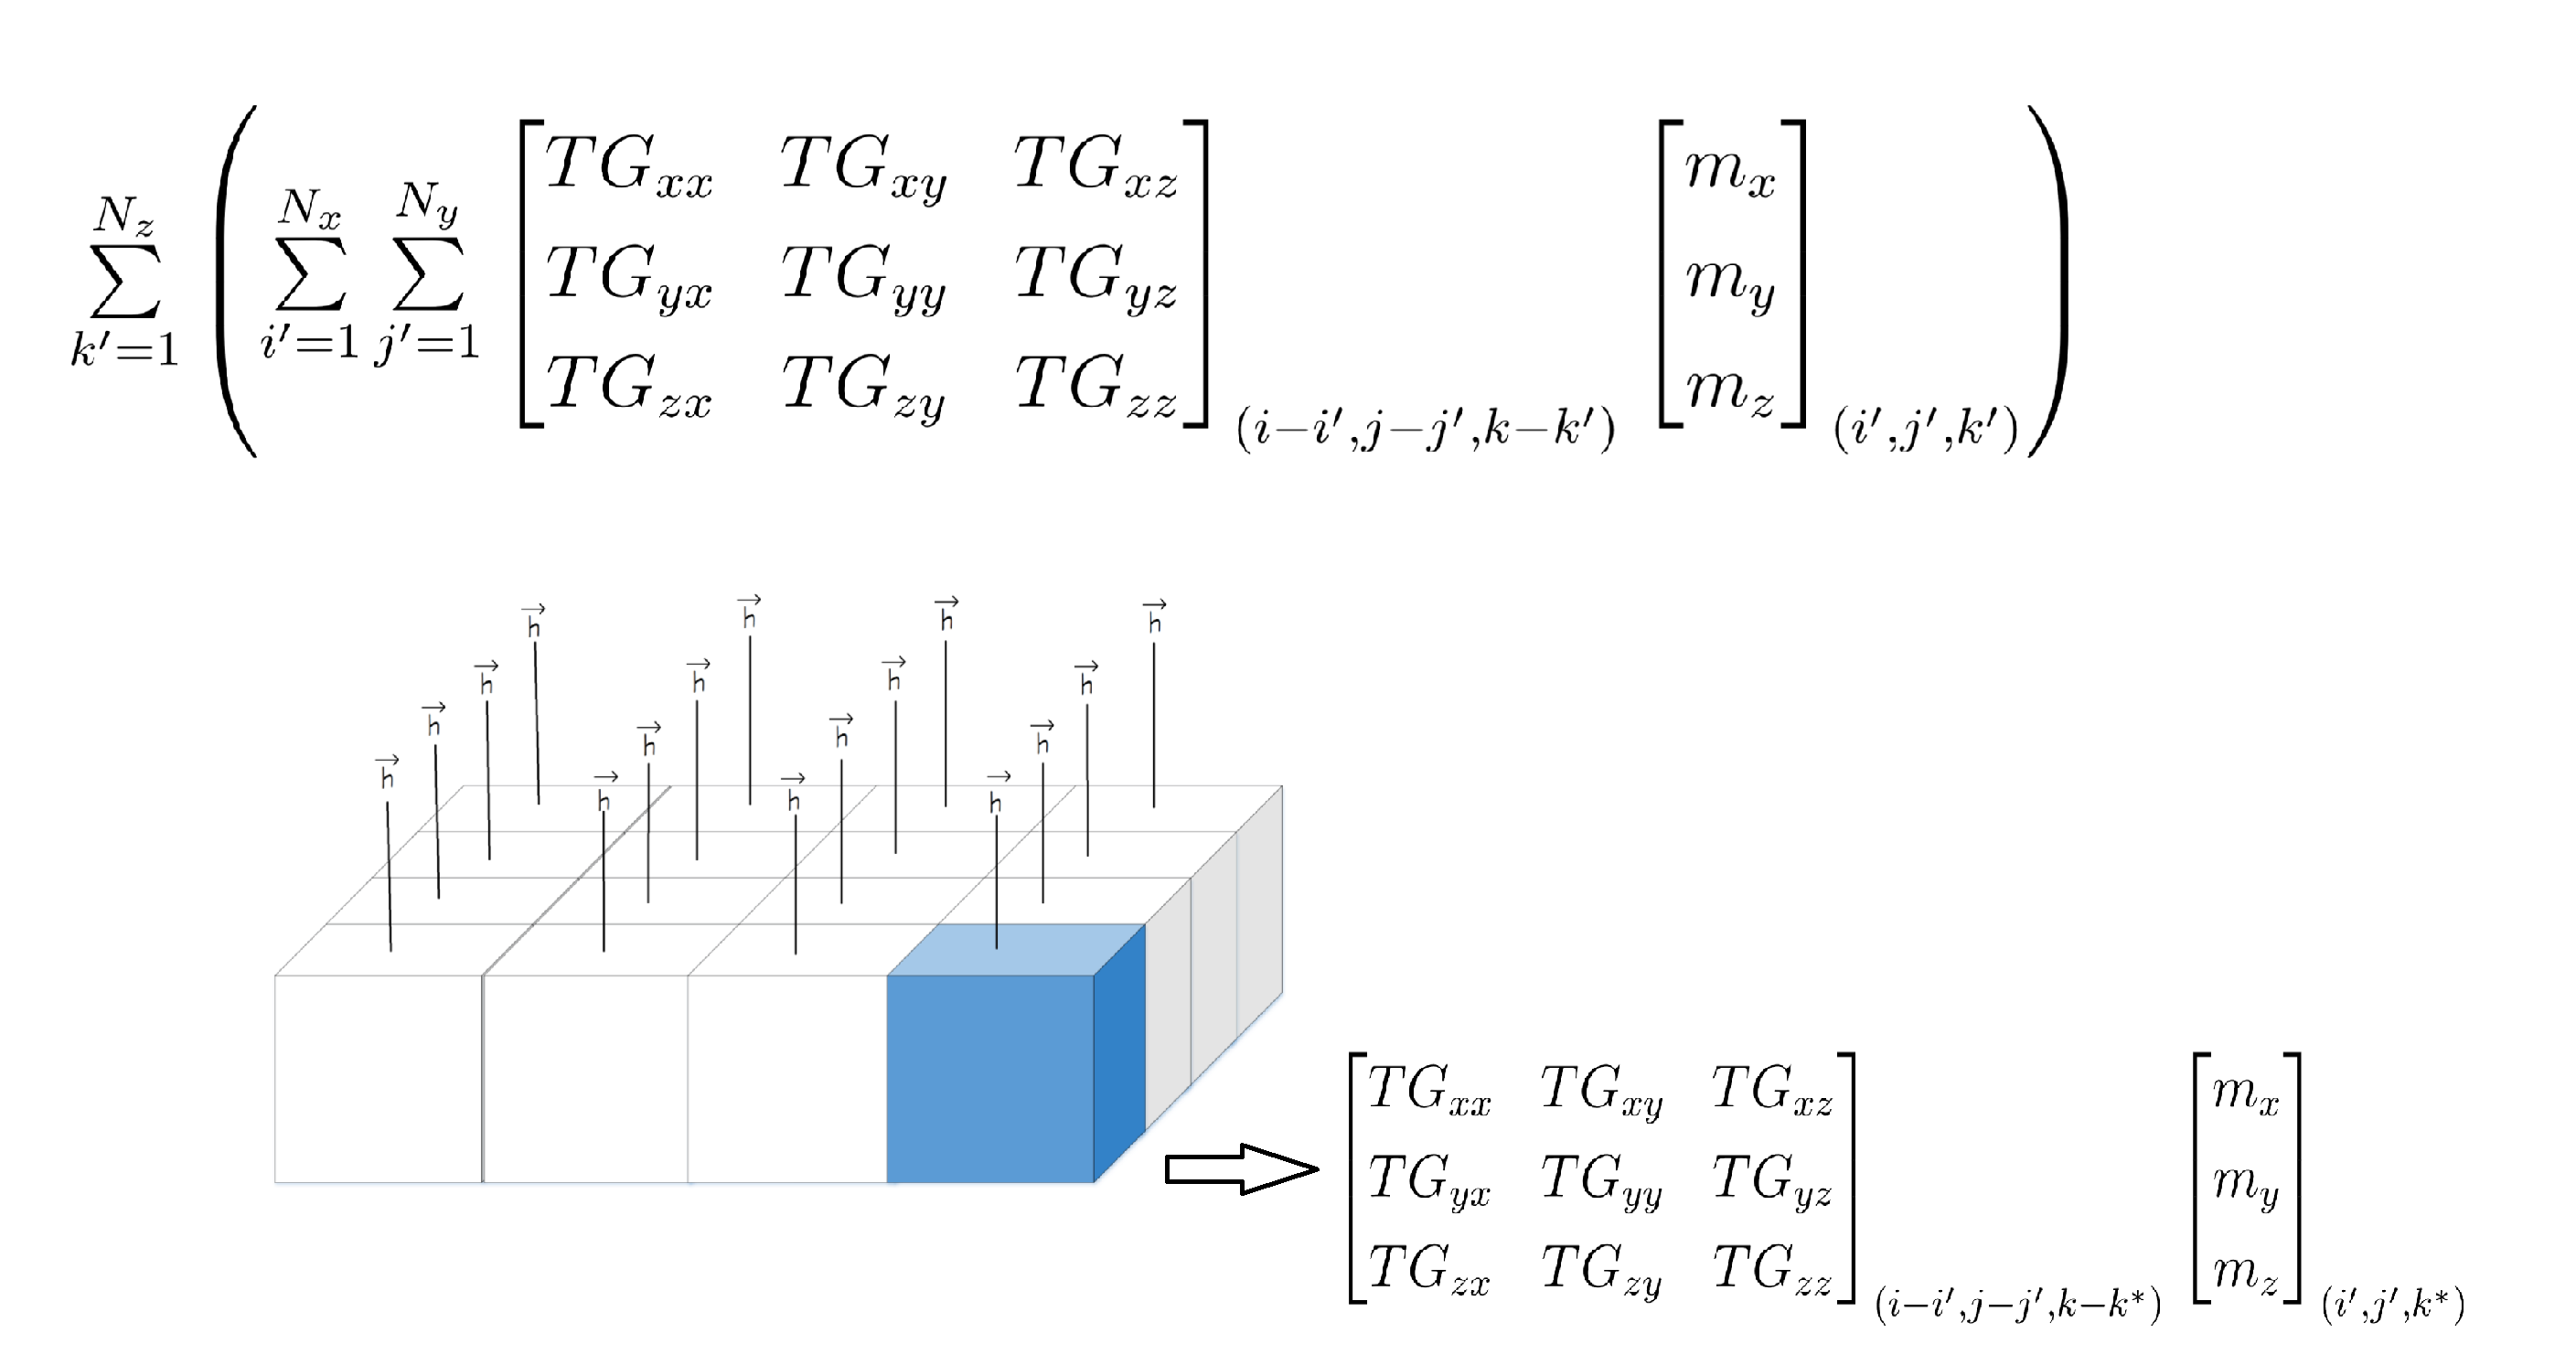
\includegraphics[width=\textwidth]{imm/3d.png}  
%	\caption{A section of the Magnetostatic field calculation 3D, where each cell perform the same operation and then we sum all the results} 
%	\label{3dpreview}
%\end{figure}
 	
	 
	
\end{document}
